\documentclass[a4paper,11pt]{article}

\usepackage{aas_macros}

\usepackage[utf8]{inputenc}	
\usepackage[T1]{fontenc}
\usepackage{lmodern}
\usepackage{times}
\usepackage[margin=2cm]{geometry}
\usepackage{amsmath,amssymb}
\usepackage{mathtools}
\usepackage{graphicx}
\usepackage{multirow}
\usepackage{blindtext}
\usepackage{hyperref}
\usepackage{float}

\usepackage{pgfplotstable} 
\usepackage{booktabs}
% \pgfplotsset{compat=1.18}


\graphicspath{ {./images/} }

\usepackage[czech]{babel}
\usepackage{graphicx}
\usepackage{xspace}
\usepackage{url}
\usepackage{indentfirst}
\usepackage{subcaption}
\usepackage{caption}
\usepackage{tabularx}
\usepackage{rotating}
\usepackage{tikz}
\usepackage[labelformat=parens,labelsep=quad,skip=3pt]{caption}

\usepackage{color}  
\usepackage{listings}

\definecolor{codegreen}{rgb}{0,0.6,0}
\definecolor{codegray}{rgb}{0.5,0.5,0.5}
\definecolor{codepurple}{rgb}{0.58,0,0.82}
\definecolor{backcolour}{rgb}{0.95,0.95,0.92}

\lstdefinestyle{mystyle}{
    backgroundcolor=\color{backcolour},   
    commentstyle=\color{codegreen},
    keywordstyle=\color{magenta},
    numberstyle=\tiny\color{codegray},
    stringstyle=\color{codepurple},
    basicstyle=\ttfamily\footnotesize\centering,        
    breaklines=true,                 
    captionpos=b,                                  
    numbers=left,                    
    numbersep=5pt,                  
    showspaces=false,              
    showstringspaces=false,
    showtabs=false,                  
    tabsize=2
}

\lstset{style=mystyle}


\widowpenalty 10000 \clubpenalty 10000 \displaywidowpenalty 10000
\setcounter{topnumber}{3}	  
\setcounter{bottomnumber}{3}	 
\setcounter{totalnumber}{6}	  
\renewcommand\topfraction{0.9}	 
\renewcommand\bottomfraction{0.9} 
\renewcommand\textfraction{0.1}	  
\intextsep=8mm \textfloatsep=8mm 

\renewcommand{\thesection}{\arabic{section}.}
\renewcommand{\thesubsection}{\thesection\arabic{subsection}.}
\makeatletter \def\@seccntformat#1{\csname the#1\endcsname\hspace{1ex}} \makeatother


\begin{document}

\noindent\hrulefill 
\begin{center}
\bigskip
\huge Určení rychlosti ztráty hmoty HD 30641 ($\alpha$ Cam)
\vspace{0.5cm}
\par \large F7581 Praktická astrofyzika - základy
\par \large Artem Gorodilov
\vspace{0.5cm}
\par \large 1. ~prosince 2024
\bigskip
\end{center}
\noindent\hrulefill 
\bigskip

\vskip10pt
    \begin{minipage}[t]{0.5\textwidth} 
        \section{Abstrakt}    
            V této práci jsem testoval různé metody výpočtu teoretické rychlosti ztráty hmoty hvězdy HD 30641 ($\alpha$ Cam). Spektralní typ hvězdy je O9.5Ia. Použité metody byly navrženy v článku \cite{2000A&A...362..295V} a porovnal jsem je s literárními údaji. Pokusil jsem se také použít metodu popsanou v článku \cite{2001A&A...369..574V}, ale neměl jsem k tomu dostatek dat.  
            \par Kromě toho jsem určil, kdy je hvězda viditelná v Brně.
            \par Výpočty byly provedeny pomocí skriptu v Pythonu\textsuperscript{\cite{github}}.

        \section{Teorie}
            \subsection{Rychlost ztráty hmoty a parametry hvězdy}
                Radiací poháněné větry v těchto hvězdách vytvářejí šoky vlivem jevu známého jako nestabilita způsobená liniovým pohonem. Tyto šoky zahřívají plyn, což vede ke vzniku rentgenového záření. Vyzařované rentgenové paprsky jsou však zároveň ovlivněny absorpcí uvnitř větru, přičemž tato absorpce hraje klíčovou roli při určování rychlosti ztráty hmoty hvězdy.
                \par V článku \cite{2000A&A...362..295V} byly navrženy dvě metody výpočtu rychlosti ztráty hmoty hvězdy. 
                \par První metoda ukazuje vztah mezi logaritmem rychlosti ztráty hmoty, svítivostí hvězdy, hmotností hvězdy, vztahem mezi terminální rychlostí a efektivní únikovou rychlostí a efektivní teplotou hvězdy: 
                \begin{equation}
                    \begin{aligned}
                        \log \dot{M} = & - (6.697 \pm 0.061) \\
                        & + (2.194 \pm 0.021) \log (L_*/10^5) \\
                        & - (1.131 \pm 0.046) \log (M_*/30) \\
                        & - (1.226 \pm 0.037) \log \left(\frac{v_{\infty}/v_{\text{esc}}}{2}\right) \\
                        & + (0.933 \pm 0.064) \log (T_{\text{eff}}/40000) \\
                        & - (10.92 \pm 0.90) \log (T_{\text{eff}}/40000)^2
                    \end{aligned}
                \end{equation}
    \end{minipage}
    \hspace{10pt}
    \begin{minipage}[t]{0.5\textwidth} 
                kde $L_*$ je svítivost hvězdy, $M_*$ je hmotnost hvězdy, $v_{\infty}$ je terminální rychlost větru, $v_{\text{esc}}$ je efektivní úniková rychlost a $T_{\text{eff}}$ je efektivní teplota hvězdy. Tento vztah a fitovací koeficienty platí pro hvězdy s teplotami: 27500 K < T$_{\text{eff}}$ < 50000 K.
                \par Druhá metoda nám umožňuje určit rychlost ztráty hmoty pomocí charakteristické hustoty větru, která je dána vzorcem:
                \begin{equation}
                    \langle \rho \rangle = \frac{\dot{M}}{8 \pi R_*^2 v_{\infty}}
                \end{equation}
                kde $R_*$ je poloměr hvězdy. Logaritmus charakteristické hustoty lze zjistit ze vztahu:
                \begin{equation}
                    \log \langle \rho \rangle = - (14.94 \pm 0.54) + (3.2 \pm 2.2) \Gamma_e
                \end{equation}
                kde $\Gamma_e$ je poměr mezi gravitačním a radiačním zrychlením.
                \par Je však třeba vzít v úvahu, že tento vztah platí pro interval teplot 22.5 kK $\lesssim$  T$_{\text{eff}}$ $\lesssim$ 26 kK. V tomto intervalu dochází k tzv. bi-stabilnímu skoku, který je pozorován při terminální rychlosti $v_{\infty}$ $\simeq$ 2.6 $v_{\text{esc}}$ \textsuperscript{\cite{2000ASPC..204..427V}}.

            \subsection{Metalicita hvězdy}
                Kromě toho jsem chtěl otestovat metodu navrženou v článku \cite{2001A&A...369..574V}. V něm byl výpočet rychlosti ztráty hmoty proveden pomocí metalicity hvězdy. Pro horkou stranu bi-stabilního skoku (27500 K < T$_{\text{eff}}$ $\leq$ 50000 K.) vypadá předpis následovně: 
                \begin{equation}
                    \begin{aligned}
                        \log \dot{M} = & - (6.697 \pm 0.061) \\
                        & + (2.194 \pm 0.021) \log (L_*/10^5) \\
                        & - (1.131 \pm 0.046) \log (M_*/30) \\
                        & - (1.226 \pm 0.037) \log \left(\frac{v_{\infty}/v_{\text{esc}}}{2}\right) \\
                        & + (0.933 \pm 0.064) \log (T_{\text{eff}}/40000) \\
                        & - (10.92 \pm 0.90) \log (T_{\text{eff}}/40000)^2 \\
                        & + (0.85 \pm 0.10) \log (Z/Z_{\odot})
                    \end{aligned}
                \end{equation}
    \end{minipage}
\newpage 
    \begin{minipage}[t]{0.5\textwidth} 
                Nebo pomocí vzorce (2):
                \begin{equation}
                    \begin{aligned}
                        \log \langle \rho \rangle = & - (14.94 \pm 0.54) \\
                        & + (0.85 \pm 1.0) \log (Z/Z_{\odot}) \\
                        & + (3.2 \pm 2.2) \Gamma_e
                    \end{aligned}
                \end{equation}
                kde $Z$ je metalicita hvězdy a $Z_{\odot}$ je metalicita Slunce.
                \par Metalicita hvězdy da se určit pomocí vztahu:
                \begin{equation}
                    [Fe/H] = \log \left(\frac{Z}{X}\right)_* - 1.61 = \log \left(\frac{Z_*}{Z_{\odot}}\right)
                \end{equation}

            \subsection{Pozorovatelnost hvězdy}
                Pozorovatelnost hvězdy zjistím podle toho, že cirkumpolární hvězdy během roku nezacházejí pod obzor: 
                \begin{center}
                    $\delta_{\text{min}}$ > 90$^{\circ}$ - $\phi$
                \end{center}
                kde $\delta_{\text{min}}$ je deklinace, kdy hvězda zachází pod obzor, $\delta_{\text{pol}}$ je deklinace pólu a $\phi$ je zeměpisná šířka pozorovatele.
        \section{Data}
            \subsection{Rychlost ztráty hmoty}
                Pro výpočet rychlosti ztráty hmoty jsem použil nasledující data:
                \begin{center}
                    \begin{tabular}{c c}
                        \hline
                        Parametr & Hodnota \\
                        \hline
                        $\log L_*$ & 5.71\textsuperscript{\cite{2004A&A...413..693M}},~ 5.51\textsuperscript{\cite{1987ApJS...64..545G}} L$_{\odot}$ \\
                        
                        $M_*$ & 43\textsuperscript{\cite{1993ApJ...412..771L}} M$_{\odot}$ \\
                        $v_{\infty}$ & (1550 $\pm$ 60)\textsuperscript{\cite{1993ApJ...412..771L}} km/s \\
                        $v_{\text{esc}}$ & 640\textsuperscript{\cite{1993ApJ...412..771L}} km/s \\
                        $T_{\text{eff}}$ & 30900\textsuperscript{\cite{1993ApJ...412..771L}} K \\
                        $R_*$ & 24.9\textsuperscript{\cite{2004A&A...413..693M}},~ 19.6\textsuperscript{\cite{1987ApJS...64..545G}} R$_{\odot}$ \\

                        $\Gamma_e$ & 0.32\textsuperscript{\cite{2004A&A...413..693M}} \\
                        \hline
                    \end{tabular}
                \end{center}
                Údaje z článku \cite{1987ApJS...64..545G} jsou uvedeny za předpokladu, že hvězda je utíkající.

            \subsection{Pozorovatelnost hvězdy}
                Hvězda $\alpha$ Cam je viditelná v souhvězdí Kameleonu. Její souřadnice jsou: 
                \begin{center}
                    $\alpha$ = 04$^{\text{h}}$ 54$^{\text{m}}$ 03.011$^{\text{s}}$, ~~ $\delta$ = +66$^{\circ}$ 20' 33.634''
                \end{center}
                Koordinaty Brna jsou:
                \begin{center}
                    $\phi$ = 49$^{\circ}$ 11' 42.79''N, ~~ $\lambda$ = 16$^{\circ}$ 36' 28.66''E
                \end{center}
    \end{minipage}
    \hspace{10pt}
    \begin{minipage}[t]{0.5\textwidth}
        \section{Vysledky}
            \subsection{Rychlost ztráty hmoty}
                Po výpočtech podle modelu (1) jsem získali následující hodnoty $\dot{M}$:
                \begin{center}
                    $\dot{M}$ = (1.53 $\pm$ 0.28) $\times$ 10$^{-6}$ M$_{\odot}$ yr$^{-1}$
                    \vspace{5pt}
                    \par $\dot{M}_{\text{runaway}}$ = (6.38 $\pm$ 1.61) $\times$ 10$^{-9}$ M$_{\odot}$ yr$^{-1}$
                \end{center}
                \par Výpočty podle modelu (2), (3) poskytly tyto výsledky:
                \begin{center}
                    $\langle \rho \rangle$ = (1.21 $\pm$ 2.48) $\times$ 10$^{-14}$ g cm$^{-3}$
                    \vspace{5pt}
                    \par $\dot{M}_{\text{bi-stab}}$ = (2.93 $\pm$ 5.99) $\times$ 10$^{-7}$ M$_{\odot}$ yr$^{-1}$
                    \vspace{5pt}
                    \par $\dot{M}_{\text{bi-stab, runaway}}$ = (1.74 $\pm$ 3.56) $\times$ 10$^{-7}$ M$_{\odot}$ yr$^{-1}$
                \end{center}
                \par Histogram je zobrazen na obrázku (\ref{fig:hist}).
            \subsection{Pozorovatelnost hvězdy}
                Deklinace, kdy hvězda $\alpha$ Cam zachází pod obzor, je:
                \begin{center}
                    $\delta_{\text{min}}$ = 40$^{\circ}$ 48' 17.21'' > 90$^{\circ}$
                \end{center}
                \par Hvězda je tedy cirkumpolární a je viditelná po celý rok v noci v Brně.
        \section{Závěr}
            Porovnáním výsledků, které jsem získal, s literárními údaji: 
            \begin{center}
                $\dot{M}_{\text{H}\alpha}$ = 4.2\textsuperscript{\cite{2004A&A...413..693M}} $\times$ 10$^{-6}$ M$_{\odot}$ yr$^{-1}$
                \vspace{5pt}
                \par $\dot{M}_{\text{H}\alpha,\text{runaway}}$ = 2.9\textsuperscript{\cite{2004A&A...413..693M}} $\times$ 10$^{-6}$ M$_{\odot}$ yr$^{-1}$
                \vspace{5pt}
                \par $\dot{M}_{\text{radio flux}}$ = (3.89 $\pm$ 1.61)\textsuperscript{\cite{1993ApJ...412..771L}} $\times$ 10$^{-6}$ M$_{\odot}$ yr$^{-1}$
                \vspace{5pt}
                \par $\dot{M}_{\text{H}\alpha}$ = (3.39 $\pm$ 1.40)\textsuperscript{\cite{1993ApJ...412..771L}} $\times$ 10$^{-6}$ M$_{\odot}$ yr$^{-1}$
                \vspace{5pt}
                \par $\dot{M}_{\text{H}\alpha}$ = (3.5 $\pm$ 0.3)\textsuperscript{\cite{1981ApJ...248.1021O}} $\times$ 10$^{-6}$ M$_{\odot}$ yr$^{-1}$
                \vspace{5pt}
                \par $\dot{M}_{\text{Metalicita}}$ = 6.04\textsuperscript{\cite{2007A&A...473..603M}} $\times$ 10$^{-6}$ M$_{\odot}$ yr$^{-1}$
            \end{center}
            je vidět, že teoretické výsledky se liší o 1-3 řády od údajů získaných pozorováním.
            \par Během posledních patnácti let se objevila řada náznaků, že predikce od Vinka a kol. nejsou v souladu s pozorováními, a to nad rámec očekávaných nejistot. Modely Vinka a kol. předpovídají ztrátu hmoty u mnoha těchto hvězd přibližně $\thicksim$ 1-2 $\times$ 10$^{-6}$ M$_{\odot}$ yr$^{-1}$, zatímco různé diagnostické metody (včetně rentgenových, UV a optických měření) tyto odhady snižují o faktor 2-3\textsuperscript{\cite{2006A&A...454..625P}}. Příkladem je hvězda $\zeta$ Ori, kde teoretická hodnota je $\dot{M}_{\text{teor}}$ = 1.2 $\times$ 10$^{-6}$ M$_{\odot}$ yr$^{-1}$, zatímco pozorovaná hodnota je výrazně nižší, $\dot{M}_{\text{obs}}$ = (3.4 $\pm$ 0.6) $\times$ 10$^{-7}$ M$_{\odot}$ yr$^{-1}$. Příčina této nesrovnalosti zůstává neznámá.
    \end{minipage}
        

\newpage
    \begin{figure}[H]
        \centering
        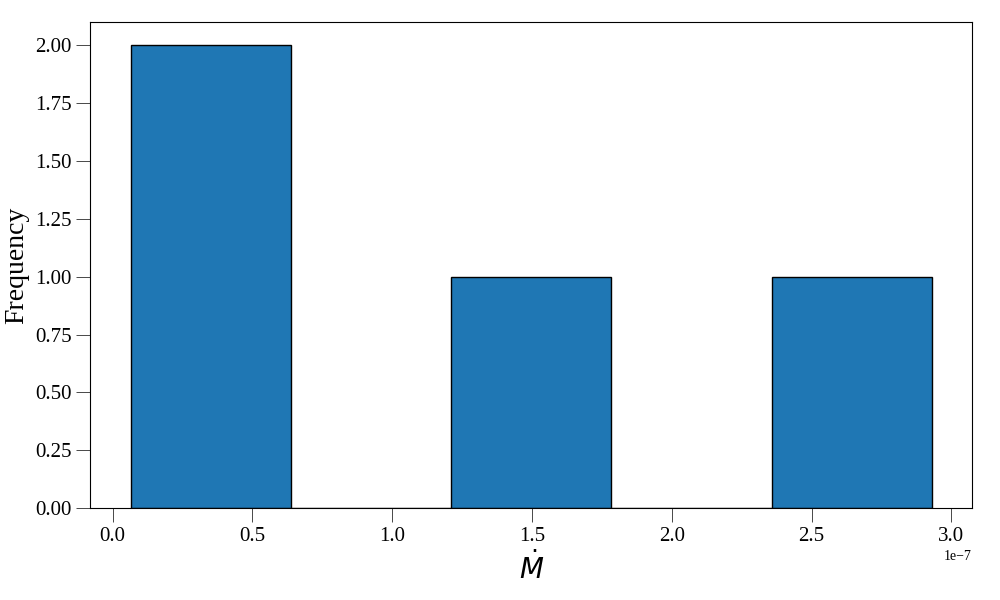
\includegraphics[scale=0.5]{hist}
        \captionsetup{justification=centering, font=footnotesize}
        \caption{Histogram rychlosti ztráty hmoty}
        \label{fig:hist}
    \end{figure}

    \bibliographystyle{plain}
    \nocite{*}
    \bibliography{refs/github, refs/vink2000, refs/vink2001, refs/vink2000b, refs/markova, refs/gies, refs/henny, refs/olson, refs/mokiem, refs/puls}

\end{document}